\documentclass[a4paper,11pt,twoside]{article}
\usepackage[german]{babel}
\usepackage[utf8]{inputenc}
\usepackage[T1]{fontenc}
\usepackage[svgnames]{xcolor}
\usepackage{amsmath, amsfonts, amssymb, graphicx, flafter, multirow, fancyhdr}
\usepackage[pdftex, colorlinks=true,linkcolor=DarkBlue, urlcolor=black, citecolor=DarkGreen]{hyperref}
\pagestyle{fancy}
\fancyhf{}
\fancyhead[L]{{\small FOPRA - Physics Simulation with Geant4}}
%%\fancyhead[C]{{\small Lorenz Schlechter, \\Thomas Kraetzschmar}}
\fancyhead[R]{{\small\date{\today}}}
\fancyfoot[C]{\thepage}
\pagestyle{fancy}
\renewcommand{\topfraction}{0.9}
\renewcommand{\bottomfraction}{0.6}
\renewcommand{\textfraction}{0.1}
\setcounter{topnumber}{3}
% Title Page
\title{%
{\Huge Physics Simulation with Geant4}\\[0.5\baselineskip]
{\normalsize Gruppe 51}
}
\author{%
Thomas Kraetzschmar
\and Lorenz Schlechter
\and Maximilian Ziegler
}
\date{\today}
%#############################################################################
\begin{document}
\pagestyle{fancy}
\pagenumbering{roman}
\maketitle
\clearpage
%\cleardoublepage
\tableofcontents
\clearpage
\pagestyle{fancy}
\pagenumbering{arabic}
%*************************************************************************************
\section{Introduction}

\section{Messung}
\subsection{Versuchsaufbau}
Um später die Genauigkeit der Simulation bestimmen zu können, wurde zuerst der simulierte Aufbau tatsächlich umgesetzt. Hierbei wurde eine Na-22 Quelle verqwendet. Diese zerfällt in einem $\beta^+$-Zerfall zu einem angeregten $^{22}Ne$, welches durch Emission eines Photons in den Grundzustand übergeht. Dieses Photon hat eine Energie von 1275 keV. Darüber hinaus kann das bei  dem $\beta^+$-Zerfall entstandene Positron mit einem Hüllenelektron annihilieren, wobei zwei Photonen der Energie 511 keV entstehen.
Diese Photonen werden mittels Caesiumiodid-Szintillationskristallen detektiert. \\\\Die Detektoren werden dabei auf vier verschiedene weisen platziert:
\begin{enumerate}
\item Die Quelle befindet sich in 3,5cm Höhe über dem Tisch, eine kleine Detektorbox befindet sich im Abstand von 3cm dazu, wobei sich der Detektorkristall 1cm tief in der Box befindet. Der Gesamtabstand beträgt damit 4cm.
\item Gleicher Aufbau nur mit einem Abstand von 5cm bzw. einem Gesamtabstand von 6 cm.
\item Die Quelle befindet sich in 3,5cm Höhe und 3cm vor der großen Detektorbox.
\item Die Quelle befindet sich in 3,5cm Höhe, auf der einen Seite befindet sich der kleine Detektor im Abstand von 5 cm, auf der anderen Seite der große Detektor im gleichen Abstand.
\end{enumerate}
Die ersten beiden Messungen dauerten 7 Minuten, die Dritte 9 Minuten und die Vierte 25 Minuten.
\subsection{Aktivität}
Die Aktivität der Probe wurde am 1.11.2013 zu $A_0=213 kBq$ bestimmt. Der Versuch wurde am 23.10.2014 durchgeführt, was einer Zeitdifferenz t von 357 Tagen entspricht. Die Halbwertszeit $T_{1/2}$ beträgt 2,6 Jahre. Damit beträgt die Aktivität zum Versuchszeitpunkt:

\begin{equation}
A=A_0*0,5^{t\over T_{1/2}}=164,11 kBq
\end{equation}

\subsection{Auswertung}
Die Messungen liefern die Anzahl der Ereignisse pro Kanal. Physikalisch interessant ist allerdings die Energie. Da die Energie der Peaks bekannt ist kann man damit den Kanälen Energien zuordnen. Dies muss für jeden Kristall einmal durchgeführt werden. Bei der ersten Messung mit dem kleinen Kristall liegen die Peaks bei den Kanälen $4316,6\pm0,4$ und $10572\pm2$. Die Peaks entsprechen den Energien 511keV und 1275keV. 
Damit lässt sich folgendermaßen eine Zuordnung berechnen:
\begin{align}
E=m*K+t\\
m={{1275keV-511keV}\over{P_2-P_1}}\\
t=511keV-P_1*m
\end{align}
Wobei $P_1$ und $P_2$ die Postionen der Peaks sind.Damit ergibt sich die Zuordnung für den Kristall in der kleinen Detektorbox:
\begin{equation}
E=0,12214*K-16,288
\end{equation}
Wobei K die Kanalnummer ist.
Wendet man diese Zuordnung auf das Spektrum der ersten messung an ergibt sich das in \ref{l1} dargestellte Spektrum.
\begin{figure}[htbp]
	\begin{center}
		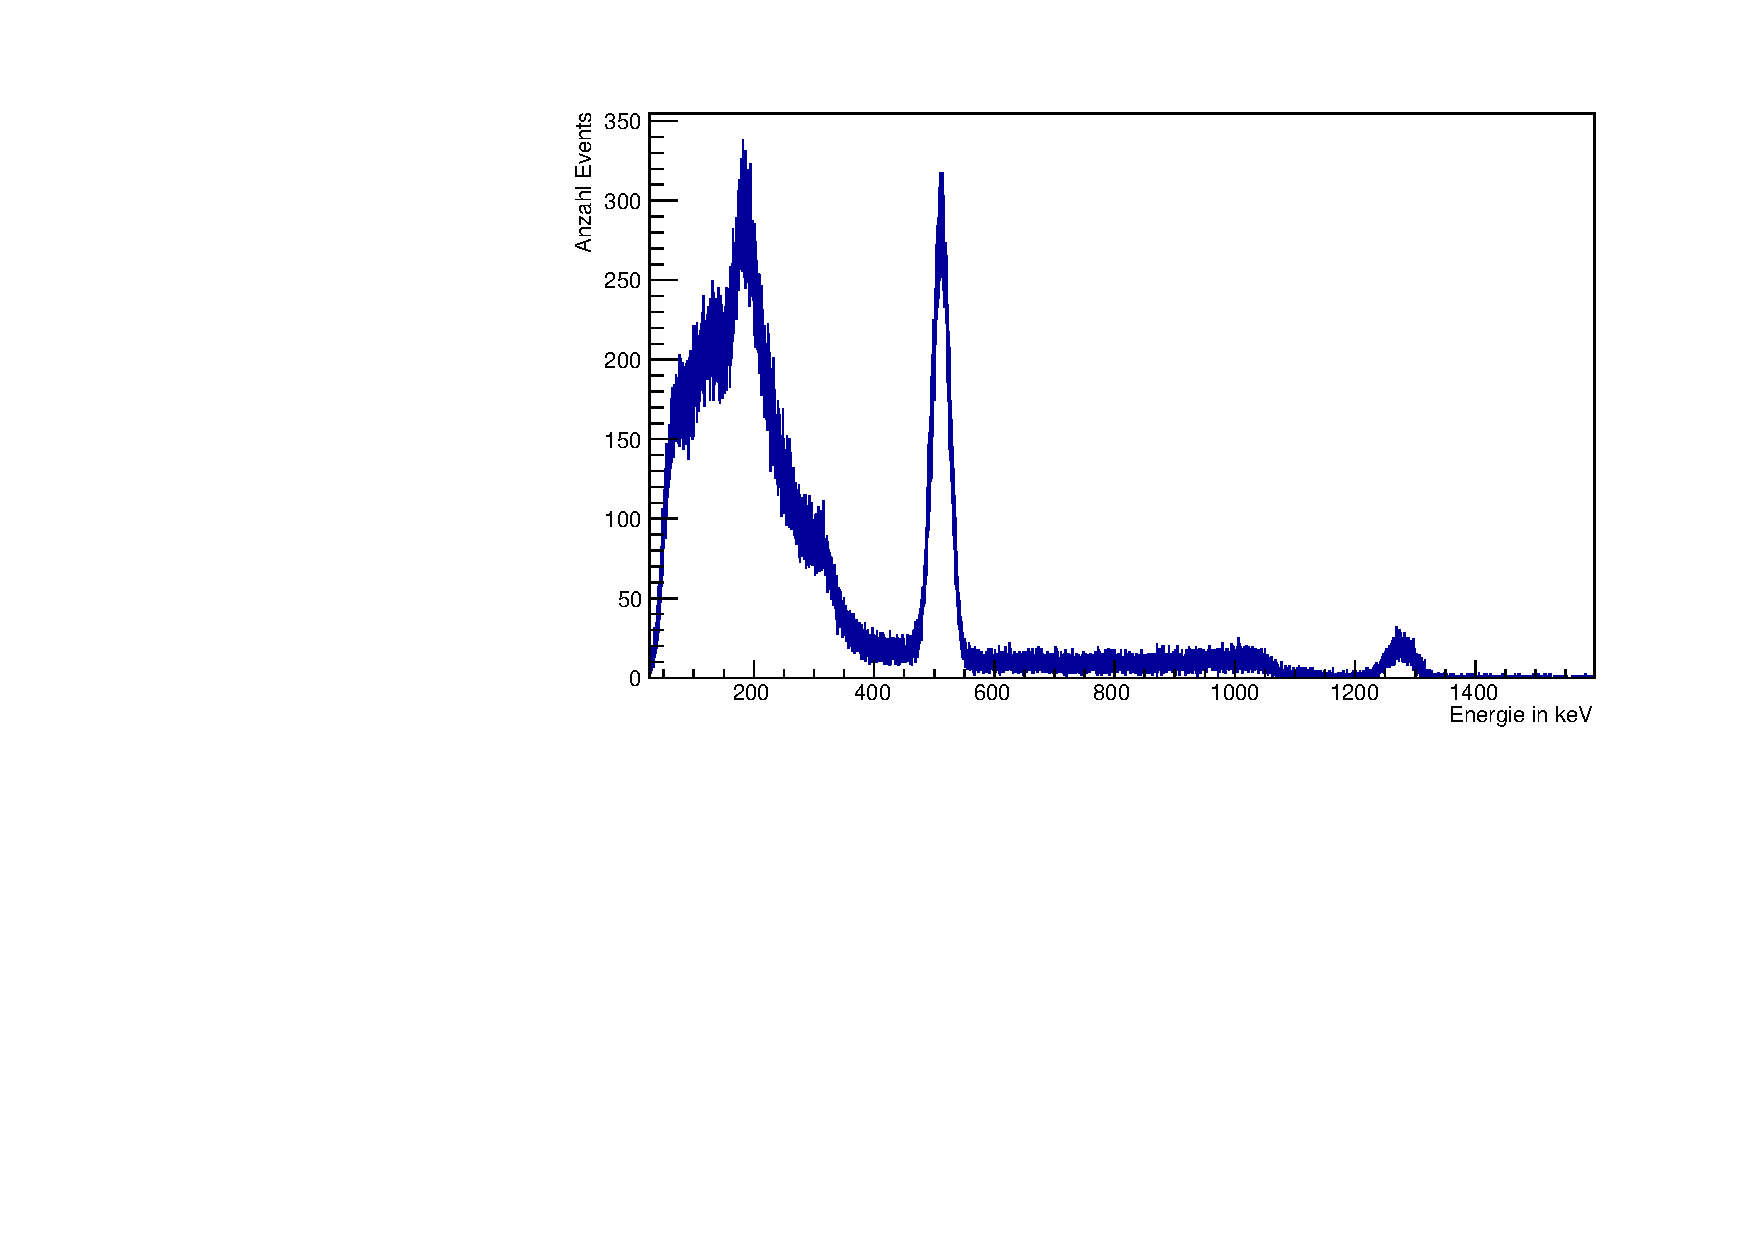
\includegraphics[width=\textwidth]{Messung11.pdf}
		\caption{Spektrum der 1. Messung}
		\label{l1}
	\end{center}
\end{figure}
Analog ergeben sich aus der dritten Messung für die beiden Kristalle der großen Detektorbox die Zuordnungen:
\begin{align}
E=0,47307*K-30,65\\
E=0,59225*K-116,78
\end {align}
Die damit erhaltenen Spektren befinden sich der Übersicht wegen im Anhang.

Um die Auflösung der Detektoren zu bestimmen werden die Peaks über eine Gaußkurve angenähert. Die Auflösung wird als Halbwertsbreite definiert, die bei einer Normalverteilung bei 1,35$\sigma$ liegt. Damit ist die Auflösung 1,35$\cdot\sigma$. Die große Detektorbox wird hierfür als ein Detektor angesehen, die Events und Varianzen der beiden Kristalle werden linear addiert, die Standardabweichung ergibt sich damit als
\begin{equation}
\sigma_{Gesamt}=\sqrt{\sigma_1^2+\sigma_2^2}
\end{equation}

\begin{figure}[htbp]
	\begin{center}
		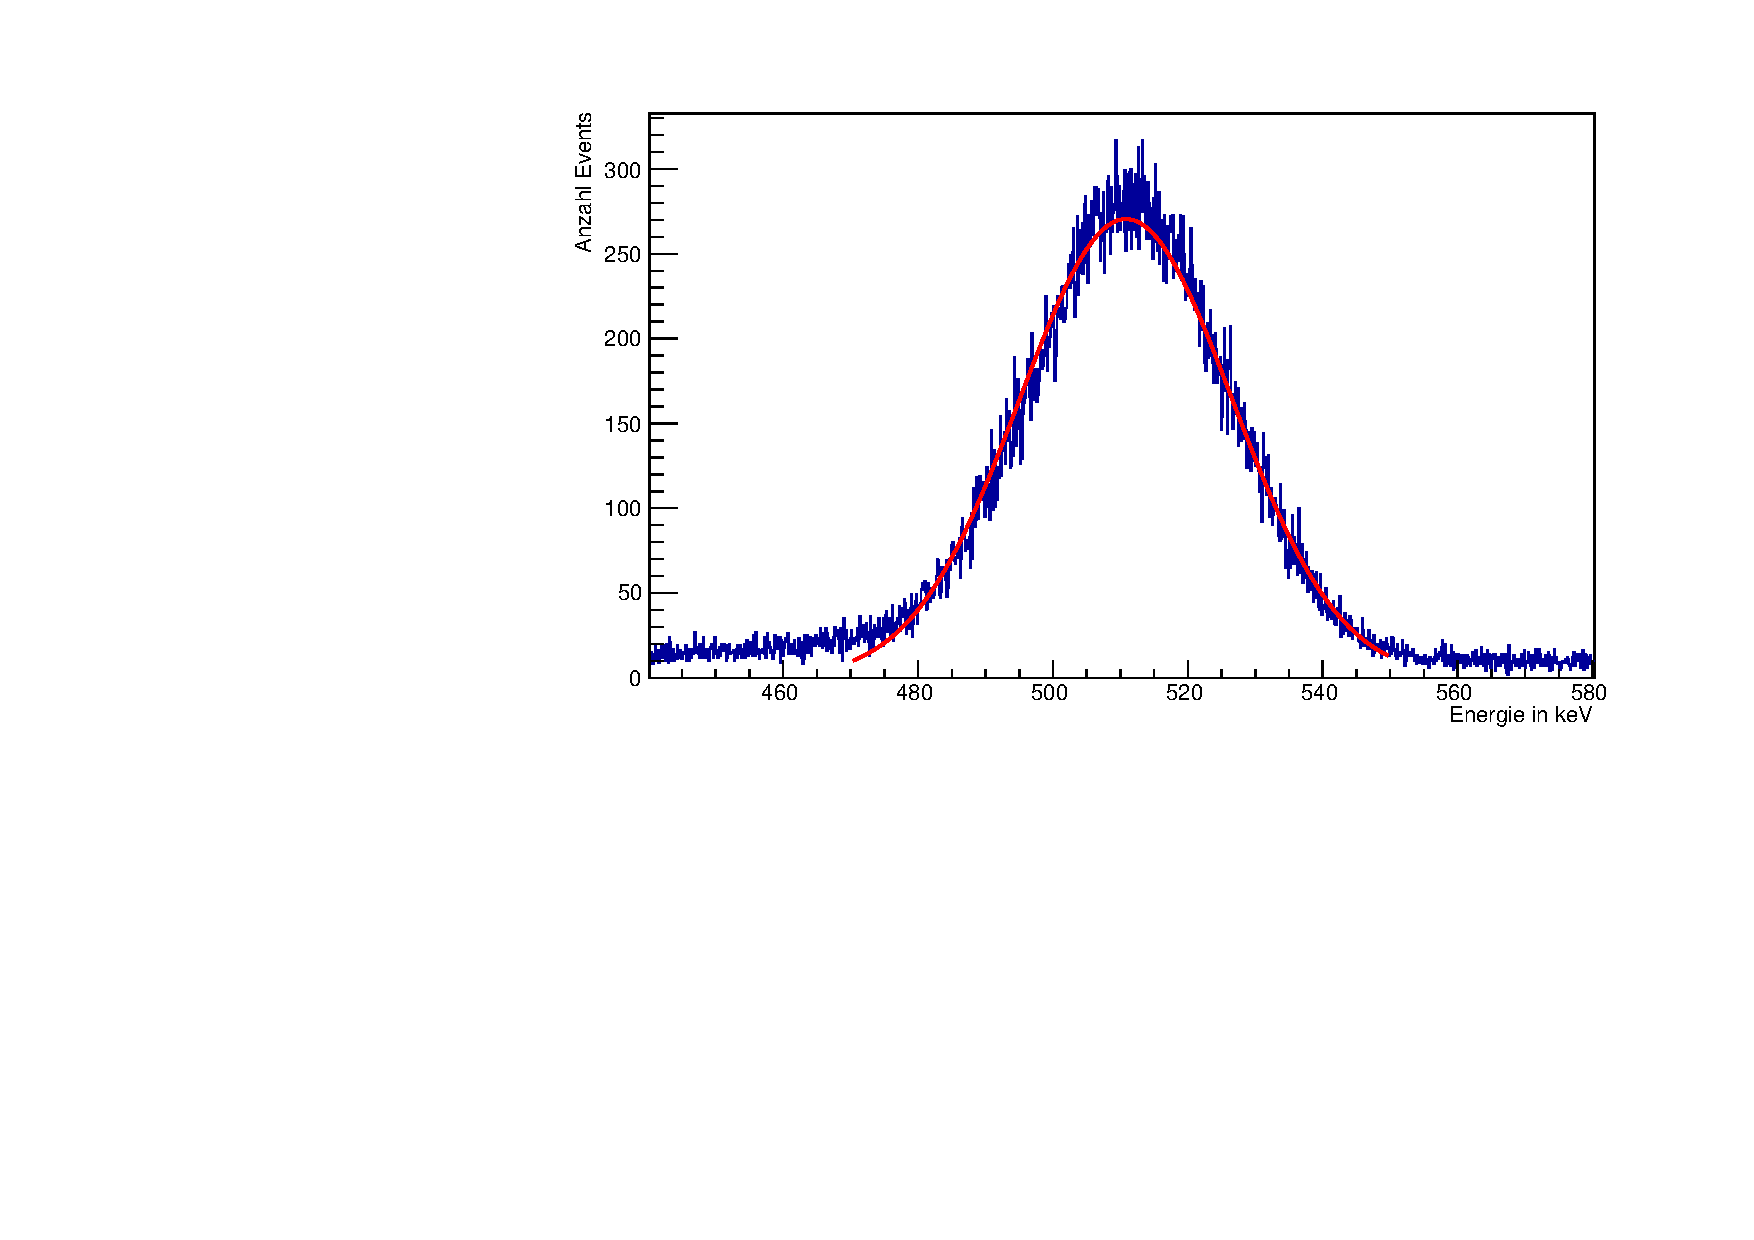
\includegraphics[width=\textwidth]{Fit1.pdf}
		\caption{Gaußscher Fit des 511 keV Peaks der ersten Messung}
		\label{l2}
	\end{center}
\end{figure}
Die Auflösung hängt neben dem Detektor auch von der Energie der einfallenden Strahlung ab.Abbildung \ref{l2} zeigt beispielhaft einen solchen Fit. Die Tabelle \ref{l3} zeigt die Ergebnisse aller Messungen.

\begin{table}
\begin{center}
    \caption{Auflösung der Detektoren}
    \label{l3}
    \begin{tabular}[c]{|c|c|c|}
    \hline
    Messung & Auflösung bei 511 keV in keV&Auflösung bei 1275 keV in keV \\
	\hline 
     1 & 21,29 & 30,16\\\hline
     2 & 20,9 & 31,3\\\hline
     3 & 85,01 & 91,99\\\hline
     
    
    \hline
    \end{tabular}
\end{center}
\end{table}
 Die Abweichungen zwischen den ersten beiden Messungen zeigen den Messfehler, da die geometrischen Effekte bereits herausgerechnet sind sollten diese Werte übereinstimmen.

\begin{table}
\begin{center}
    \caption{Effizienzen der Detektoren}
    \label{l4}
    \begin{tabular}[c]{|c|c|c|c|c|}
    \hline
    Messung & $\eta_{geometrisch}$&$\eta_{Photopeak}$ bei 511 keV &$\eta_{Photopeak}$ bei 1275 keV \\\hline 
     1 & 0,6\% & 10,57\%&2,15\%\\\hline
     2 & 0,27\% & 12,8\%&2,43\%\\\hline
     3 &3,75\% & 2,74\%&0,92\%\\\hline
     
    
    \hline
    \end{tabular}
\end{center}
\end{table}
Die Effizienz setzt sich zusammen aus der geometrischen Effizienz und der Detektoreffizienz. Die geometrische Effizienz ist der Anteil des gesamten Raumwinkels den der Detektor abdeckt und wird über folgenden Ausdruck genähert:
\begin{equation}
\eta_{geometrisch}={A\over 4 \pi d^2}
\end{equation}
Die Photopeakeffizienz ergibt sich damit als
\begin{equation}
\eta_{Photopeak}={N_{peak}\over N_0\cdot\eta_{geometrisch}}
\end{equation}
Wobei $N_0$ die Anzahl der emitierten Photonen ist, die sich aus der Aktivität ergibt. Hierbei ist zu beachten, dass bei der Annihilierung eines Elektrons mit einem Positron 2 $\gamma$-Quanten entstehen. Der kleine Detektor besteht aus einem Kristall der Frontfläche $A=121mm^2$. Der Wert für die Kirstalldimensionen wurde aus der Simulation ausgelesen. Bei der ersten Messung betrug der Abstand zur Detektorbox 3cm, der Gesamtabstand zwischen Quelle und Detektorkristall also 4cm. Damit ergibt sich eine geometrische Effizienz von 0,602\%. Zusammen mit der Aktivität von 164,11kBq, 87710 Events sowie der Messzeit von 7 Minuten ergibt sich eine Photopeakffizienz von
\begin{equation}
\eta_{Photopeak}={87710\over 2\cdot7\cdot60\cdot164110\cdot0,0602}=10,57\%
\end{equation}
Analog lassen sich alle anderen Effizienzen berechnen, Tabelle\ref{l4} zeigt die Ergebnisse. Erneut zeigt der Unterschied zwischen den ersten beiden Messungen die Messungenauigkeit.
%\bibliographystyle{alpha}
%\bibliographystyle{apalike}
%\bibliographystyle{plain}
%\bibliography{Literaturverzeichniss-Brue}
%\appendix
\begin{figure}[htbp]
	\begin{center}
		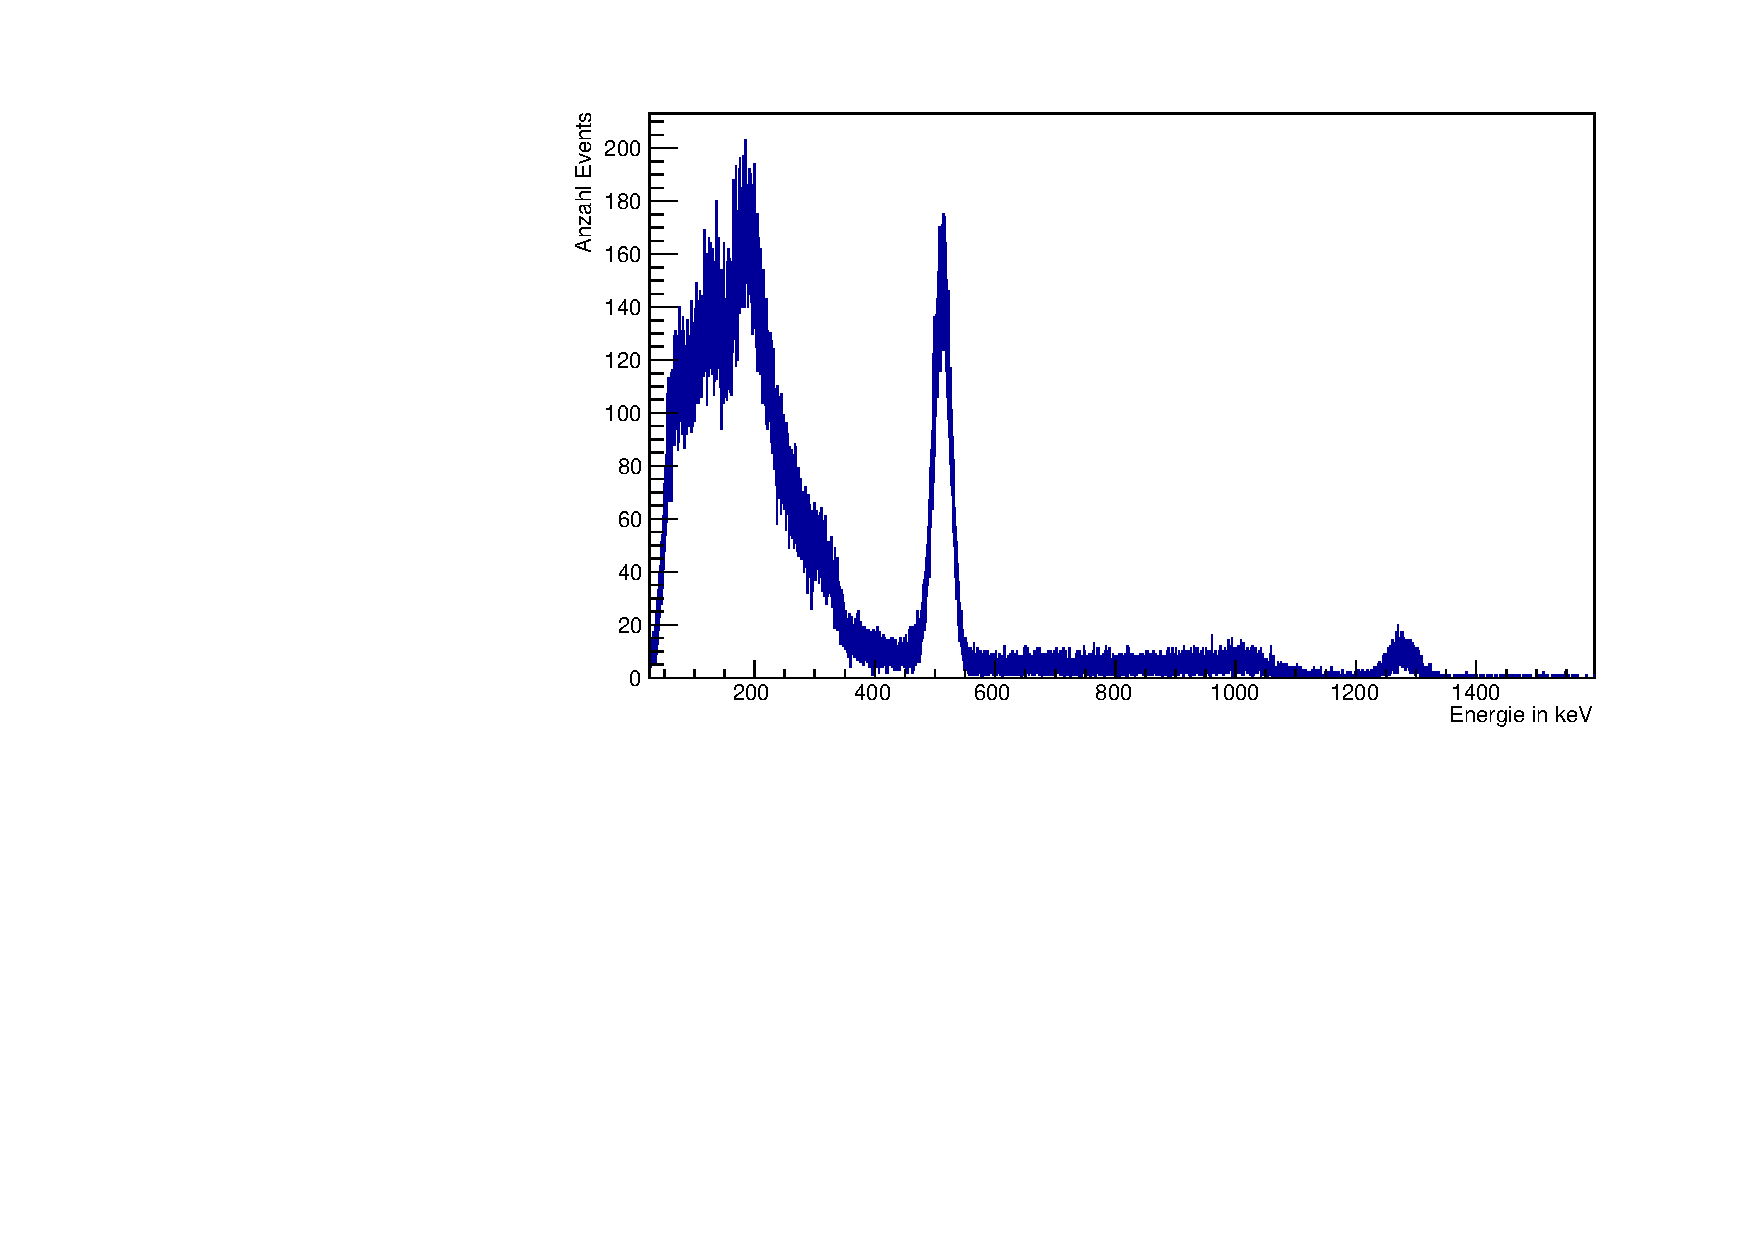
\includegraphics[width=\textwidth]{Messung2.pdf}
		\caption{Spektrum aus Messung 2}
		
	\end{center}
\end{figure}
\begin{figure}[htbp]
	\begin{center}
		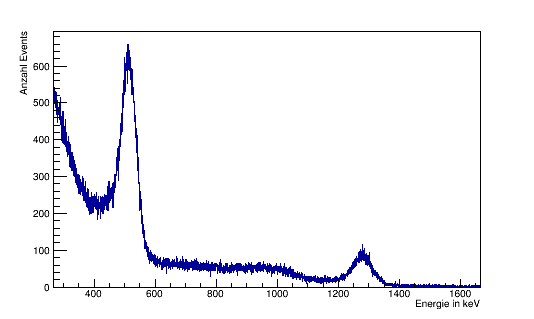
\includegraphics[width=\textwidth]{Messung31.png}
		\caption{Spektrum erster Kristall aus Messung 3}
		
	\end{center}
\end{figure}
\begin{figure}[htbp]
	\begin{center}
		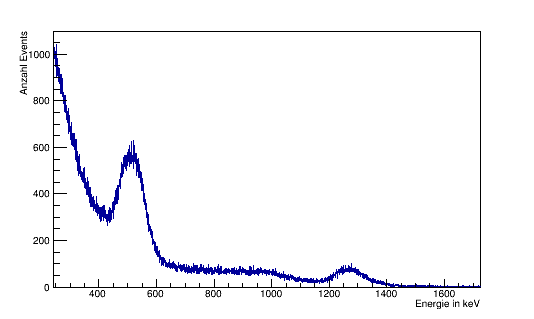
\includegraphics[width=\textwidth]{Messung32.png}
		\caption{Spektrum zweiter Kristall aus Messung 3}
		
	\end{center}
\end{figure}


%\listoffigures
%\listoftables
%
\end{document} 